%!TEX root = main.tex

\newpage
\chapter{Informačné bulletiny}

Informačné bulletiny (angl. \emph{newsletters}) sú aj v súčasnosti jedným z najrozšírenejších spôsobov, ako v online
prostredí informovať používateľov o dianí na webovom portáli. Prevádzkovatelia webových portálov využívajú informačné
bulletiny na predstavenie nového obsahu, akciového tovaru, zaujímavostí z určitej oblasti alebo špeciálnych ponúk pre
svojich používateľov a zákazníkov. Informačné bulletiny sú tiež využívané ako prostriedok pre motiváciu používateľov
k opätovnej návšteve webového portálu.

Informačné bulletiny spravidla nadobúdajú formu e-mailu, ktorý je zvyčajne v pravidelných intervaloch doručovaný
do schránok používateľov, ktorí o jeho doručovanie prejavili záujem.


\section{Problémy informačných bulletinov}
Hlavným problémom informačných bulletinov v súčasnosi je stále sa znižujúva miera interakcie používateľov
s informačnými bulletinmi.

Štúdia spoločnosti Silverpop z roku 2012~\cite{mailmarketing} na vzorke informačných bulletinov 1124 spoločností ukázala,
že počet používateľov, ktorí vôbec otvoria informačný bulletin sa pohybuje na úrovni 20\% a stále klesá. Navyše konkrétne
v oblasti technológií sa táto hodnota pohybuje len na 16,5\%. Ešte menšia je miera preklikov
(angl. \emph{Click-through rate - CTR}), ktorá sa celkovo pohybuje na úrovni 5,4\% a v prípade technologicky zameraných
informačných bulletinov len 3,6\%. Napriek tomu sa miera odhlásení z odoberania (angl. \emph{unsubscribe rate}) pohybuje
len na úrovni 2\%.

Dôvodov, prečo používatelia prejavujú iba malý záujem o informačné bulletiny ktoré im sú doručované, môže byť niekoľko.
Jedným z takýchto dôvodov môže byť vysoká saturácia -- používateľom chodí priveľké množstvo informačných bulletinov,
dôsledkom čoho používatelia rezignujú a tieto e-maily ani neotvárajú.
Hlavným nedostatkom informačných bulletinov, a zároveň dôvodom, prečo iba 5\% používateľov klikne na obsah v informačnom
bulletine, je však relevancia ponúkaného obsahu.


\section{Relevancia v informačných bulletinoch}

Množstvo webových portálov doručuje všetkým svojim používateľom presne ten istý obsah informačného bulletinu.
Často je tento obsah vytváraný manuálne editormi, a zameriava sa len všeobecne na aktuálne dianie na danom webovom
portáli. Takýto všeobecný informačný bulletin však nutne nemôže byť dostatočne relevantný pre značnú časť používateľov.

Riešením problému relevancie infromačných bulletinov je vytváranie personalizovaných informačných bulletinov, ktoré
každému používateľovi ponúkajú len ten obsah, ktorý je pre neho najzaujímavejší a najrelevantnejší.


\section{Informačné bulletiny v CQA systémoch}

Význam informačných bulletinov značne narastá aj v rámci online komunít, ktoré produkujú veľké množstvo používateľmi
vytváraného obsahu. Medzi prominentné druhy takýchto online komunít patria aj systémy pre odpovedanie na otázky
(angl.~\emph{Community Question Answering - CQA}).

Súčasný výskum v oblasti CQA systémov~\cite{Srba2016} sa venuje predovšetkým oblastiam skúmania správania používateľov,
smerovania a odporúčania otázok a kvality otázok a odpovedí v týchto systémoch. Problematike vytvárania informačných
bulletinov v doméne CQA systémov zatiaľ nebola venovaná veľká pozornosť.

Mnohé populárne CQA systémy aj v súčasnosti ponúkajú svojim používateľom informačné bulletiny majúce iba generický
charakter a nijakým spôsobom neuvažujú relevantnosť obsahu pre konkrétnych používateľov, prípadne informačné bulletiny
neponúkajú vôbec.

\subsection{Informačné bulletiny v sieti Stack Exchange}

Sieť Stack Exchange\footnote{ \url{https://stackexchange.com}}, ktorá patrí medzi najpopulárnejšie CQA systémy súčasnosti,
sa skladá z viac ako 160 samostatných komunít zameraných na rôzne oblasti. Stack Exchange ponúka používateľom všetkých
komunít možnosť odoberať informačný bulletin, ktorý je doručovaný raz týždenne.

Informačné bulletiny komunít Stack Exchange obsahujú tri sekcie (Obr.~\ref{fig:so-newsletter}). Prvá sekcia je rovnaká
pre všetkých používateľov konkrétnej komunity a obsahuje zoznam najlepšie hodnotených nových otázok.
Obsah nasledujúcich dvoch sekcií je náhodne generovaný. Tieto sekcie obsahujú najpopulárnejšie otázky z predchádzajúceho
týždňa a náhodný výber nezodpovedaných otázok.

Používatelia CQA systému Stack Exchange nie sú s takýmto generickým informačným bulletinom
spokojní~\footnote{ \url{https://meta.stackoverflow.com/q/336925}. Prevzaté 30.4.2017.}\footnote{
\url{https://meta.stackexchange.com/q/247298}. Prevzaté 31.4.2017.}.
Generický informačný bulletin stráca pre používateľov informačnú hodnotu, pretože
najmä v prípade väčších komunít, akou je napríklad Stack Overflow\footnote{ \url{https://stackoverflow.com}}, často obsahuje
otázky, ktoré nie sú z oblastí záujmu používateľa. Najviac sa tento problém prejavuje na sekcii nezodpovedaných otázok.
Tie sú vyberané náhodne, takže pravdepodobnosť, že používateľ vie na niektorú z nich odpovedať, je malá.


\begin{figure}[H]\begin{center}
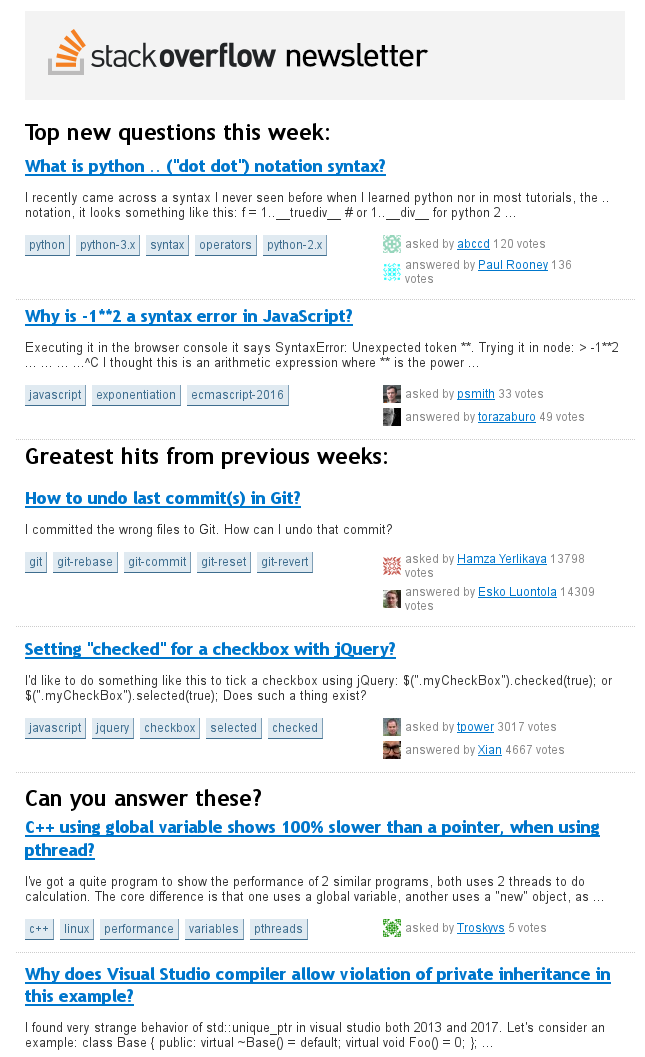
\includegraphics[scale=0.4]{so-newsletter}
\caption{Informačný bulletin komunity Stack Overflow, 25. apríl 2017.\label{fig:so-newsletter}}\end{center}
\end{figure}

\subsection{Informačný bulletin portálu Quora}

Quora\footnote{\url{https://quora.com}} je CQA systém, ktorý nie je zameraný na konkrétnu oblasť záujmu, ale obsahuje
otázky z rôznych tém. Quora ponúka svojim používateľom týždenný informačný bulletin (\emph{Quora Weekly Digest}),
ktorý obsahuje desať najzaujímavejšich otázok za posledný týždeň a zoznam ľudí, ktorých používateľ potenciálne pozná.

Zoznam najzaujímavejších otázok pozostáva z editormi manuálne vybraného obsahu a algoritmicky vybraného obsahu,
ktorý je personalizovaný pre každého používateľa zvlášť (Obr.~\ref{fig:quora-newsletter}).

\begin{figure}[H]\begin{center}
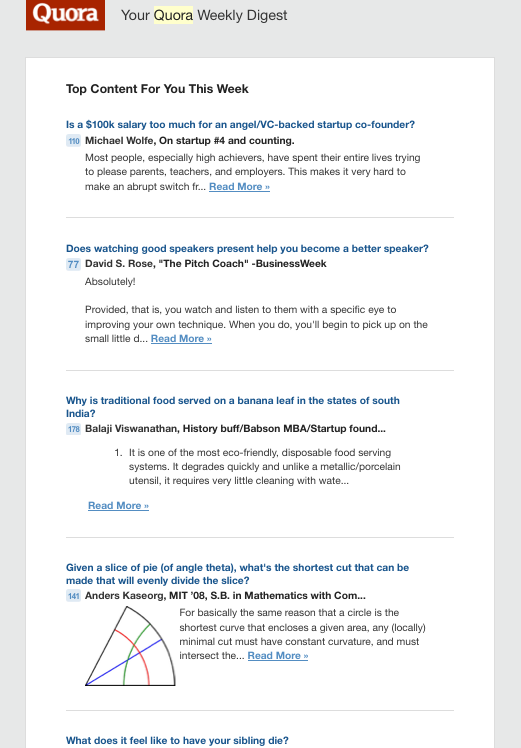
\includegraphics[scale=0.5]{quora-newsletter}
\caption{Informačný bulletin portálu Quora. Prevzaté 30.4.2017, \url{http://www.businessinsider.com/quora-emails-2012-8}
\label{fig:quora-newsletter}}\end{center}
\end{figure}

\subsection{CQA systémy bez informačných bulletinov}

Viaceré populárne CQA systémy svojim používateľom vôbec neponúkajú možnosť odoberať informačný bulletin. Medzi takéto
systémy patrí napr. portál \emph{Yahoo! Answers}\footnote{\url{https://answers.yahoo.com}}, ktorý je určený na pokladanie
otázok z akejkoľvek oblasti záujmu. Rovnako informačný newsletter neponúka ani ďalší všeobecne zameraný CQA systém --
\emph{Wiki Answers}\footnote{\url{https://answers.com}}. CQA systém zameraný na podporu výučby
\emph{Askalot}\footnote{\url{http://askalot.fiit.stuba.sk}} tiež v súčasnosti neponúka informačný newsletter,
iba možnosť notifikácie používateľa prostredníctvom e-mailu o aktivite súvisiacej s jeho obsahom v rámci systému.



%%%%%%%%%%%%%%%%%%%%%%%%%%%%%%%%%%%%%%%%%%%%%%%%%%%%%%%%%%%%%%%%%%%%%%%%%%%%%%%%%%%%%%%%%%%%%%%%%%%%%%%%%%%%%%%%%%%%%%%%


\newpage
\chapter{CQA systémy}

CQA systémy sú jednou z výrazných skupín webových portálov, ktoré sú založené na princípe používateľsky vytváraného obsahu.
Tieto systémy umožňujú používateľom položiť otázky, ktoré nie je možné zodpovedať použitím štandardných vyhľadávačov~\cite{Liu2012}
a zároveň odpovedať na otázky iných používateľov.

Napriek tomu, že väčšina CQA systémov sa spočiatku zameriava najmä na poskytnutie zmysluplnej odpovede na konkrétnu otázku,
v súčasnosti je možné v prípade niektorých CQA systémov (napr. Stack Overflow) vnímať postupnú zmenu zamerania
z jednorázových odpovedí na kolaboratívne vytváranie komplexnejších poznatkov s dlhodobou hodnotou~\cite{Anderson2012}.
Za týmto účelom CQA systémy implementujú hlasovanie a princíp reputácie ako spôsob podpory komunitného aspektu označovania
najlepších odpovedí na položené otázky.


\section{Problémy CQA systémov}

CQA systémy sa musia vysporiadavať s tými istými druhmi problémov, ako iné kategórie systémov založené na používateľmi
vytvorenom obsahu.

\subsection{Problém dlhého chvosta}
Čím viac sa zvýrazňuje trend orientácie CQA systémov viac na poskytovanie obsahu s dlhodobou hodnotou ako na samotné
poskytnutie odpovede na položenú otázku, tým viac sa prehlbuje problém \emph{dlhého chvosta} (angl. \emph{long tail}).
Ide o štandardný problém všetkých stránok zameriavajúcich sa na používateľmi vytváraný obsah, kedy je veľká väčšina
používateľov týchto stránok len pasívnymi čitateľmi (angl. \emph{lurkers}) a najväčšia časť obsahu je vytvorená len veľmi
úzkou skupinou najaktívnejších používateľov.

V prípade CQA systému Stack Overflow sa podiel aktívnych používateľov (takých, ktorí za sledovaný mesiac pridali
do systému aspoň jednu otázku alebo odpoveď) za marec 2017 pohyboval na úrovni 3\% všetkých
používateľov~\cite{Srba2016SOFail}\footnote{Výsledky za aktuálne obdobie boli získané prostredníctvom nástroja Stack
Exchange Data Explorer.}.

\subsection{Variabilita v kvalite obsahu}
Ďalším problémom CQA systémov je variabilná kvalita otázok a odpovedí v týchto systémoch. Zvyšujúcou sa popularitou CQA
systémov narastá aj podiel obsahu s nízkou kvalitou, či už vo forme veľmi jednoduchých otázok alebo nedostatočne
podrobných odpovedí, ako aj množstvo duplicitných otázok -- otázok, ktoré už boli v systéme
zodpovedané~\cite{Srba2016SOFail,Ponzanelli2014}.

Jedným z riešení tohto problému, ktorý využíva aj CQA systém Stack Overflow, je komunitné zabezpečovanie kvality obsahu
prostredníctvom moderátorov -- používateľov s oprávnením upravovať, označiť duplikát alebo vymazať obsah.


\section{Druhy CQA systémov}

CQA systémy možno kategorizovať do dvoch základných skupín podľa toho, na akú oblasť otázok sa tieto systémy zameriavajú.

\subsection{Univerzálne CQA systémy}

CQA systémy ako \emph{Yahoo! Answers}, \emph{Wiki Answers} alebo \emph{Quora} nie sú zamerané na konkrétne oblasti
a umožňujú používateľom pokladať otázky na akékoľvek témy~\cite{Chua2014}.

Tento druh CQA systémov má štandardne vyšší počet používateľov aj aktivity ako úzko špecializované CQA systémy,
no tiež tu existuje väčšia pravdepodobnosť výskytu nekvalitných, jednoduchých alebo neužitočných otázok a odpovedí,
ako aj veľký počet duplicitných otázok, ktoré už boli zodpovedané. Zároveň sú univerzálne CQA systémy zameriané viac
na samotný proces kladenia otázok a odpovedania na ne, než na vytváranie dlhodobo hodnotného obsahu.

\subsection{Úzko špecializované CQA systémy}

Opakom univerzálnych CQA systémov sú CQA systémy, ktoré sú špecializované na konkrétne oblasti záujmu.
Medzi takéto CQA systémy patria napríklad jednotlivé komunity v rámci siete Stack Exchange, ktorá zahŕňa rôzne druhy
komunít, od všeobecnejších, ako je napr. komunita venujúca sa matematike\footnote{\url{https://math.stackexchange.com}},
po veľmi úzko špecializované, akými sú napr. komunity \emph{Ask Ubuntu}\footnote{\url{https://askubuntu.com}} alebo
\emph{Raspberry Pi}\footnote{\url{https://raspberrypi.stackexchange.com}} venujúce sa konkrétnym produktom.

Tématicky zamerané CQA systémy majú väčší potenciál pre vznik dlhodobo hodnotného obsahu~\cite{Anderson2012}. V rámci
týchto systémov tiež vzniká množstvo prepojení medzi obsahom \textit{(otázky podobného charakteru, riešenie problému
v príbuznej oblasti)}, čo vedie k vzniku \emph{znalostných sietí}~(angl.~\emph{knowledge networks})~\cite{Li2016}.
S cieľom zvýšiť hodnotu jednotlivých príspevkov tiež mnohé CQA systémy zavádzajú možnosť komunitnej úpravy
otázok a odpovedí~\cite{Li2015}, čo vedie okrem zvýšenej aktivity aj k zvýšeniu vnímanej užitočnosti príspevku.



%%%%%%%%%%%%%%%%%%%%%%%%%%%%%%%%%%%%%%%%%%%%%%%%%%%%%%%%%%%%%%%%%%%%%%%%%%%%%%%%%%%%%%%%%%%%%%%%%%%%%%%%%%%%%%%%%%%%%%%%


\chapter{Odporúčanie}

\section{Odporúčacie systémy}

Odporúčacie systémy sú softvérové nástroje a techniky ktoré používateľom ponúkajú položky, ktoré by pre nich mohli
byť nejakým spôsobom zaujímavé alebo užitočné~\cite{Handbook2011}. Tieto odporúčania sú zvyčajne ponúkané za účelom
pomôcť používateľovi rozhodnúť sa, aké články by si mal prečítať, alebo aký tovar si kúpiť.

Využívanie odporúčacích systémov je tiež pre používateľov vhodným spôsobom, ako zvládať problémy informačného zahltenia
v dnešnom online svete. Ako také sa odporúčacie systémy stávajú jedným z najsilnejších a najpopulárnejších nástrojov
v online komunitách.

Odporúčacie systémy typicky vytvárajú zoznam odporúčaní jedným z dvoch spôsobov -- buď prostredníctvom \emph{kolaboratívneho
filtrovania} (angl.~\emph{Collaborative filtering}), alebo použitím \emph{filtrovania založeného na obsahu}
(angl.~\emph{Content-based filtering})~\cite{Buhmann2011}. Tieto dva prístupy môžu byť tiež kombinované
v hybridných odporúčacích systémoch.

\subsection{Kolaboratívne filtrovanie}\label{rec:collab}

Odporúčacie systémy využívajúce kolaboratívne filtrovanie fungujú prostredníctvom získavania spätnej väzby používateľa
vo forme hodnotení pre položky v danej doméne a využívajú podobnosti v hodnotení medzi viacerými používateľmi na určenie
či určitý obsah odporučiť, alebo nie~\cite{Buhmann2011}. Metódy kolaboratívneho filtrovania možno ďalej rozdeliť
na metódy založené na susednosti alebo na základe modelu.

Kolaboratívne filtrovanie na základe susednosti (angl.~\emph{Neighborhood-based Collaborative filtering})
vyberá skupinu používateľov podľa ich podobnosti k aktuálnemu používateľovi
a použitím váženej kombinácie ich hodnotení vyberá odporúčaný obsah pre tohto používateľa.
Techniky založené na modeli (angl.~\emph{Model-based Collaborative filtering}) poskytujú odporúčania prostedníctvom
oceňovania parametrov štatistických modelov pre používateľské hodnotenia.

\subsection{Filtrovanie na základe obsahu}\label{rec:content}

Odporúčanie čisto prostedníctvom kolaboratívneho filtrovania využíva iba používateľské hodnotenia. Tieto prístupy berú
všetkých používateľov a položky ako atomické jednotky a odporúčania sú vytvárané bez ohľadu na konkrétne špecifiká
individuálnych používateľov alebo položiek.

Metódy využívajúce filtrovanie na základe obsahu naopak vytvárajú
odporúčania na základe porovnávania modelov reprezentujúcich obsah s modelmi reprezentujúcimi konkrétneho používateľa.
Odporúčania v takýchto prístupoch vznikajú na základe prekryvu týchto dvoch modelov.


\section{Odporúčanie v CQA systémoch}

V kontexte CQA systémov je problematika odporúčania a odporúčacích systémov častým objektom výskumu~\cite{Srba2016}.

Jedným z hlavných cieľov CQA systémov je poskytnúť pýtajúcemu sa odpoveď na jeho otázku v čo možno najkratšom čase.
Rovnako ako v prípade iných systémov založených na používateľmi vytváranom obsahu, aj v prípade CQA systémov miera
nového obsahu -- nových otázok a odpovedí -- neustále narastá. Napriek tomu je tiež možné pozorovať stúpajúci trend
nízkej miery zodpovedanosti otázok~\cite{Srba2016SOFail}. Jedným zo spôsobov, ako je možné riešiť túto situáciu,
je práve využitie odporúčacích systémov.

V súčasnosti jedným z trendov najmä v úzko zameraných CQA systémoch ako napr. Stack Overflow, je tiež postupný prechod
od modelu jednoduchého odpovedania na položené otázky na model povzbudzujúci k vytváraniu dlhodobo hodnotného obsahu
vo forme rozsiahlych komunitne spravovaných odpovedí~\cite{Anderson2012,Li2015} podnecujúcich diskusiu.
V tomto prípade je možné využiť odporúčacie systémy ako prostriedok pre odhalenie a prezentovanie otázok a odpovedí,
ktoré by mohli používateľa zaujímať a priniesť mu úžitok~\cite{Toba2014} aj v prípade, že práve nemá rovnaký problém,
ako sa vyskytuje v danej otázke.

Výskum v oblasti odporúčania v CQA systémoch sa v súčasnosti zameriava hlavne na oblasti odporúčania, smerovania
a získavania otázok. Problémom súčasného výskumu v tejto oblasti je nejednoznačnosť a časté zamieňanie týchto výrazov,
prípadne nerozlišovanie medzi odporúčaním a smerovaním otázok~\cite{Srba2016}.

\subsection{Odporúčanie otázok}

Odporúčanie otázok (angl.~\emph{Question recommendation}) využíva tzv. \emph{pull} prístup, teda na základe (explicitnej
či implicitnej) požiadavky používateľa prezentuje zoznam odporúčaných relevantných otázok (alebo obsahu celkovo).
Tento prístup využíva štandardnejší tok medzi použitými modelmi -- začína sa modelom používateľa, na ktorý sa odporúčací
systém pokúša namapovať model relevantného obsahu.
Relevancia otázok pre používateľa môže byť identifikovaná rôznymi prístupmi -- či už na základe kolaboratívneho
filtrovania (\ref{rec:collab}) alebo filtrovania na základe obsahu (\ref{rec:content}).

Forma prezentovania odporúčaných otázok sa tiež môže líšiť. Časté je napríklad zobrazenie príbuzných otázok v detaile
konkrétnej otázky, ktorú moementálne používateľ číta. Odporúčanie otázok je však možné využiť aj ako prostriedok pre
zvýšenie záujmu a angažovanosti používateľa o CQA systém.


\subsection{Smerovanie otázok}

Na rozdiel od pomerne štandardného odporúčania otázok, v prípade smerovania otázok (angl.~\emph{Question routing})
je prístup k odporúčaniu presne opačný, a využíva tzv. \emph{push} prístup. V tomto prípade proces odporúčania začína
modelom nezodpovedanej otázky, ktorú sa snaží odporúčací systém nasmerovať k používateľovi, ktorý má najväčší potenciál
na túto otázku zodpovedať.

Výskum smerovania nezodpovedaných otázok na konkrétnych používateľov -- odpovedajúcich -- síce ukazuje, že ide o dôležitý
koncept aj z pohľadu používateľského zážitku~\cite{Li2010,Li2011}, no prináša so sebou aj problémy. Najvýraznejším z nich je zahltenie
expertov, ktorí sú hlavnými terčmi takejto formy odporúčania, nakoľko ich reputácia a expertíza ich predurčuje ako vhodných
kandidátov na zodpovedanie veľkého množstva otázok~\cite{Pal2015}.

Pomerne novým prístupom k smerovaniu otázok je namiesto zamerania na konkrétnych používateľov smerovanie otázok na väčšie
komunity používateľov~\cite{Liu2014}. Hlavnou ideou takéhoto smerovania je fakt, že kolektívne poznatky komunity sú vždy väčšie, ako
poznatky konkrétneho používateľa, aj experta~\cite{Pal2013}. Navyše takéto smerovanie zvyšuje pravdepodobnosť rýchlejšieho zodpovedania
otázky, ako aj zabraňuje zahlteniu expertov. Hlavným problémom smerovania na komunity je vytváranie kolektívneho modelu
reprezentujúceho komunitu, kedy je potrebné brať do úvahy okrem iného fakt, že iba malá časť komunity sú \emph{tvorcovia
poznatkov} a nie len ich konzumenti~\cite{Pal2015}.


\subsection{Získavanie otázok}

Tento pojem (angl.~\emph{Question retrieval}) v kontexte CQA systémov hovorí o procese vyberania podobných otázok pre
rôzne formy dopytov~\cite{Zhang2014} na základe syntaktickej podobnosti otázok.
Tento proces je možné využiť na hľadanie odpovedí alebo poznatkov vo veľkých množstvách už zodpovedaných otázok.


\subsection{Problém studeného štartu}

Častým problémom odporúčania je problém studeného štartu (angl.~\emph{Cold start}), kedy je na dosiahnutie primeranej
miery presnosti odporúčania potrebné veľké množstvo informácií, ktoré ale napr. v prípade nových alebo menej aktívnych
používateľov nemusia byť k dispozícii.

Tento problém sa vyskytuje najmä v prípade systémov, ktoré obsah odporúčajú na základe
podobnosti používateľov medzi sebou. Keďže je často na začiatok potrebné veľké množstvo informácií o daných používateľoch,
nie je možné jednoducho odporúčať vhodný obsah pre používateľov, ktorí sú menej aktívni, alebo sú noví.
V menšej miere týmto problémom trpia systémy, ktoré namiesto podobnosti používateľov využívajú pre zostavovanie odporúčaní
podobnosť samotného obsahu na základe rôznych atribútov.

\subsection{Segmentácia používateľov}

Ďalším z problémov v oblasti personalizovaného odporúčania, veľmi výrazným aj v prípade informačných bulletinov,
je rozdelenie používateľov zaujímajúcich sa o informačný bulletin do skupín podľa účelu, za ktorým chcú informačný bulletin dostávať.
V prípade úzko zameraných CQA systémov, ako je napr. Stack Overflow, je možné používateľov rozdeliť do dvoch základných
skupín -- producentov a konzumentov.

Producenti sú používatelia, ktorí primárne odpovedajú na otázky. Takýto používatelia
tvoria dôležitú časť komunity~\cite{Anderson2012}. Motiváciou pre odoberanie informačného bulletinu pre takýchto používateľov
je hlavne potenciál identifikovať otázky, ktoré ešte neboli dostatočne alebo správne zodpovedané, prípadne záujem
o diskusiu o zaujímavých a netriviálnych otázkach. Konzumenti sú zase používatelia, ktorí sú spravidla v rámci komunity
používateľov menej aktívni a ich motiváciou je zbierať vedomosti~\cite{Anderson2012}. Pre týchto používateľov je potrebné
identifikovať vysoko kvalitné odpovede na otázky~\cite{Toba2014}.

Jednotlivé skupiny používateľov tak prirodzene očakávajú nie len iný druh otázok, ale aj celé odlišné súčasti informačných bulletinov.


\subsection{Problém filtračnej bubliny}\label{rec:filterbubble}

Ďalším problémom, ktorému sa však v oblasti odporúčania obsahu CQA systémov venuje menej pozornosti~\cite{Srba2016},
je rôznorodosť odporúčaného obsahu. Hrozí tak výskyt problému tzv. filtračnej bubliny (angl.~\emph{Filter bubble}).

Ak totiž systém používateľovi odporúča obsah len z oblastí používateľovho záujmu, dochádza k problému, kedy je používateľ
do značnej miery uzatvorený v rámci jednej oblasti a nemá tak možnosť získavať zaujímavé poznatky z iných oblastí.
Používateľ sa tak síce môže stať odborníkom na danú oblasť, no jeho povedomie o širšom kontexte celej problematiky
je veľmi obmedzené.

Riešením tohto problému je identifikácia oblastí, ktoré nie sú priamo oblasťami záujmu používateľa, no sú k týmto
oblastiam v určitých aspektoch príbuzné. Používateľ má tak možnosť rozšíriť svoj okruh záujmu a vedomosti o širšom
kontexte problémovej domény.


%%%%%%%%%%%%%%%%%%%%%%%%%%%%%%%%%%%%%%%%%%%%%%%%%%%%%%%%%%%%%%%%%%%%%%%%%%%%%%%%%%%%%%%%%%%%%%%%%%%%%%%%%%%%%%%%%%%%%%%%


\chapter{Diverzita a aktuálnosť odporúčania}

Diverzitu možno všeobecne definovať ako opak podobnosti. V niektorých prípadoch však nemusí byť odporúčanie podobných
položiek tým najlepším riešením pre používateľa~\cite{Handbook2011}. Dôvodom je práve náchylnosť takéhoto odporúčania na
vyvolanie problému filtračnej bubliny (viď kapitola \ref{rec:filterbubble}).

Okrem diverzifikácie odporúčaného obsahu má na celkovú úspešnosť vytvárania personalizovaných odporúčaní veľký vplyv aj
aktuálnosť (angl.~\emph{freshness}, príp.~\emph{novelty}) odporúčaného obsahu~\cite{Liu2015}.

\section{Diverzita v odporúčacích systémoch}

Tématická diverzifikácia je metóda napomáhajúca vyváženosti a diverzite personalizovaného odporúčania s cieľom
lepšie reflektovať kompletné spektrum používateľových záujmov. Napriek tomu, že môže mať negatívny vplyv na priemernú
správnosť odporúčaní, dosahuje táto metdóda zvýšenú úroveň používateľskej spokojnosti~\cite{Zhang2009}.

Ziegler a kol.~\cite{Ziegler2005} študovali diverzifikáciu v oblasti odporúčaní a navrhli prístup, ktorý vytvára
zoznamy odporúčaní lepšie uspokojujúce používateľove záujmy prostredníctvom selekcie takých zoznamov, ktoré majú nízku
vnútornú podobnosť. Autori v experimente demonštrovali, že reálny používatelia preferujú diverznejšie výsledky.

Tradičný spôsob zavedenia diverzity do odporúčania je diverzifikácia na základe atribútov odporúčaného obsahu, teda
zoskupenie výsledkov do skupín zdieľajúcich viaceré atribúty (ako napr. žáner hudby) a následný výber iba limitovaného
množstva výsledkov z každej zo skupín. Autori v~\cite{Yu2009} prezentujú \emph{diverzifikáciu na základe dôvodu}.
Táto metóda využíva pre diverzifikáciu výsledkov dôvod, prečo bola konkrétna položka odporučená
(napr. \textit{tento album bol odporučený, pretože ste počúvali inú skladbu tohto autora}). Autori experimentálne ukázali,
že takáto forma diverzifikácie je prinajmenšom rovnako účinná, ako diverzifikácia na základe atribútov položiek.

Inú perspektívu volí metóda diverzity na báze proporcionality. Zoznam odporúčaní je možné považovať za najlepšie diverzifikovaný
vzhľadom na relevanciu odporúčaní v takom prípade, keď počet výsledkov z určitej témy je úmerný popularite danej témy.
Dang a kol. vo svojej práci~\cite{Dang2012} ponúkajú koncept optimalizácie proporčnosti pre diverzifikáciu výsledkov
vyhľadávania.

Napriek tomu, že sa táto práca nezaoberá priamo diverzitou v odporúčacích systémov, sú paralely s touto
oblasťou výrazné. Motiváciou pre tákyto spôsob diverzifikácie je metóda obsadzovania kresiel v parlamente. Ich metóda
postupne pre každú pozíciu v zozname výsledkov určuje tému, ktorá najlepšie zachováva celkovú proporčnosť. Následne
na túto pozíciu z danej témy vyberie najlepší dokument.


\section{Aktuálnosť v odporúčacích systémoch}

Aktuálnosť v kontexte odporúčacích systémov môže predstavovať dva rôzne aspekty. Jedným z nich je \emph{novosť}
(angl.~\emph{novelty}), teda pomerne priamočiara vlastnosť určujúca, či odporúčaný obsah už bol používateľovi prezentovaný,
alebo nie. Jednoduchým spôsobom, ako zabezpečiť, aby používateľovi neboli stále dookola odporúčané tie isté položky,
akokoľvek relevantné by pre neho mohli byť, je odfiltrovanie položiek, ktoré už používateľovi boli odporúčané v minulosti,
a s ktorými už interagoval~\cite{Handbook2011}.

Druhým aspektom aktuálnosti je \emph{čerstvosť} (angl.~\emph{freshness}). V tomto prípade ide o časovú aktuálnosť odporúčaného
obsahu. Naivný prístup k aktuálnosti je odporúčanie iba obsahu z určitého obmedzeného časového úseku z blízkej minulosti,
no takýto prístup nemusí vždy dosahovať najlepšie výsledky používateľskej spokojnosti~\cite{Szpektor2013}.

Pri odporúčaní, ktoré berie do úvahy aktuálnosť odporúčaného obsahu je dôležitým aspektom detekcia časovo citlivej témy.
Takýto systém by mal brať presadzovať aktuálny obsah iba v prípade, kedy je to vhodné. Na druhej strane, ak je v prípade
aktívne sa vyvýjajúcej témy odporúčaný neaktuálny obsah, môže to výrazne degradovať úspešnosť odporúčania~\cite{Dong2010}.
Ďalším faktorom pri posudzovaní aktuálnosti v odporúčaní je časová škála aktuálnosti pre danú tému.
V prípade niektorých tém alebo oblastí je možné považovať za aktuálne položky z posledného roka, no v iných prípadoch
môžu byť aj niekoľko týždňov staré položky považované za vysoko neaktuálne.

Ďalším problémom vzhľadom na aktuálnosť v odporúčaní je tiež fakt, že pre novo vzniknutý obsah môže byť problémovejšie
zostaviť model, ktorý by ho reprezentoval, nakoľko môže byť o tomto obsahu známych zatiaľ iba málo informácií~\cite{Dong2010TW}.
Tento problém studeného štartu sa môže prejavovať rovnako v prípade modelovania obsahu, ako je tomu napríklad v prípade
vytvárania modelov reprezentujúcich nových používateľov.

Riešením v takomto prípade môže byť napríklad vytváranie modelu
obsahu na základe čŕt, ktoré nie sú ovplyvnené časom (napr. nadpis, text alebo autor obsahu, na rozdiel od počtu hlasov
alebo dátumu uverejnenia), alebo tiež upravenie hodnôt týchto čŕt vzhľadom na relatívnu aktuálnosť obsahu.


\section{Diverzita a aktuálnosť v kontexte CQA systémov}

Kým diverzita a aktuálnosť sú v oblasti odporúčania a celkovo vo vyhľadávaní informácií pomerne často analyzovanými aspektmi,
v kontexte CQA systémov sa týmto hľadiskám doteraz venovala iba okrajová pozornosť~\cite{Srba2016}.

Liu a kol. vo svojej práci~\cite{Liu2015} skúmajú aspekt aktuálnosti odporúčania v CQA systémoch prostredníctvom
relatívne neštandardného návrhu CQA systému určeného pre odpovedanie v reálnom čase na \emph{hyper-lokálne} a časovo senzitívne
otázky. Za týmto účelom využívajú prístupy predchádzajúcich prác a kombinujú aspekty relevancie, lokality a aktuálnosti
v \emph{real-time} CQA systéme.


Komplexnejší pohľad na aktuálnosť a diverzitu priamo v kontexte štandardných CQA systémov ponúka Szpektor a kol~\cite{Szpektor2013}.
Autori experimentovali so zavedením diverzity a aktuálnosti do procesu vytvárania odporúčaní pre používateľov CQA
systému Yahoo! Answers, pričom sa na rozdiel od väčšiny prác v tejto oblasti nezameriavali len na skupinu expertných používateľov.

Pre odporúčanie využili profil otázok založený na kombinácii LDA, lexikálneho a kategorického modelu a profil používateľa
odvodený od profilu otázok, s ktorými interagoval. Párovanie otázok a používateľov bolo vykonané prostredníctvom jednoduchého
skalárneho súčinu vektorov reprezentujúcich profily používateľov a otázok.

Samotná diverzifikácia odporúčaní bola vykonávaná prostredníctvom tématického výberu vzoriek (angl.~\emph{thematic sampling}),
kedy je vygenerovaných viacero samostatných zoznamov odporúčaných otázok z viacerých tém, ktoré sú následne zmiešané dokopy
proporcionálne k pravdepodobnostnému skóre jednotlivých tématických zoznamov.

Prínos aktuálnosti do odporúčania v CQA systémoch bol skúmaný na základe odporúčania iba aktuálneho obsahu -- konkrétne
iba nezodpovedaných otázok za posledné štyri hodiny.

Dopad diverzifkácie a aktuálnosti na úspešnosť odporúčania bol testovaný v rámci online experimentu. Používatelia boli náhodne
rozdelení do štyroch segmentov:

\begin{my_enumerate}
  \item{\textbf{Kontrolná vzorka} -- Týmto používateľom neboli ponúknuté žiadne odporúčania.}
  \item{\textbf{Odporúčanie na základe relevancie} -- Používateľom boli ponúknuté odporúčania iba na základe relevancie
        daných otázok, bez ohľadu na aktuálnosť alebo diverzitu.}
  \item{\textbf{Odporúčanie s ohľadom na aktuálnosť} -- Používateľom boli odporúčané relevantné otázky, pričom 50\% z nich
        pochádzalo z posledných štyroch hodín a 20\% bolo vybraných prostredníctvom tématického výberu vzoriek.}
  \item{\textbf{Diverzifikované odporúčanie} -- Používateľom boli odporúčané relevantné otázky, pričom 50\% z nich
        bolo vybraných na základe tématického výberu vzoriek ako prostriedku diverzifikácie, a 20\% pochádzalo z posledných
        štyroch hodín.}
\end{my_enumerate}

Výsledky online experimentu potvrdili intuitívnu myšilienku, že iba samotná relevancia nie je dostatočná na úspešne
odporúčanie otázok v CQA systéme. Práve naopak, vo vykonanom experimente dokonca samotné odporúčanie len na základe
relevancie dosiahlo nižšie hodnoty zodpovedania otázok, ako kontrolná vzorka bez akýchkoľvek odporúčaní.

Presadzovanie aktuálnych otázok dosiahlo zvýšenie miery zodpovedania otázok o 4\%, avšak najlepšie výsledky boli dosiahnuté
prostredníctvom diverzifikácie odporúčaní aj za cenu zníženia aktuálnosti, pričom miera zodpovedania sa zvýšila o 17\%.

\vspace*{1.5cm}

Na základe tejto analýzy môžeme usúdiť, že napriek tomu, že problematika diverzifikácie a aktuálnosti odporúčania v kontexte
CQA systémov v súčasnosti stále ostáva do veľkej miery nepreskúmaná, je očividné, že uvažovanie týchto aspektov v tomto
kontexte má veľký vplyv na úspešnosť odporúčania, pričom informačné bulletiny sa javia ako prirodzená, požadovaná,
no napriek tomu málo využívaná forma prinášania odporúčaného a potenciálne zaujímavého obsahu použivateľom.
